% Document is compatible with XeLaTex only. Don't use PDFLaTex!

\documentclass[a4paper,10pt,ngerman]{scrartcl}
\usepackage[ngerman]{babel}
\usepackage{fontspec}
%\usepackage[utf8x]{inputenc}
\usepackage[a4paper,margin=2.5cm,footskip=0.5cm]{geometry}
\usepackage{graphicx}
%\usepackage{marvosym} % Sonderzeichen

\usepackage{algorithm}
\usepackage{algpseudocode}
\usepackage{algorithmicx}
\algrenewcommand{\Return}{\State\algorithmicreturn~} %for return in new line

% Die nächsten vier Felder bitte anpassen:
\newcommand{\Aufgabe}{Aufgabe 1: Hopsitexte}      % Aufgabennummer und Aufgabennamen angeben
\newcommand{\TeamId}{00578}                       % Team-ID aus dem PMS angeben
\newcommand{\TeamName}{Frederik Hamann}           % Team-Namen angeben
\newcommand{\Namen}{Frederik Hamann}              % Namen der Bearbeiter/-innen dieser Aufgabe angeben

% Kopf- und Fußzeilen
\usepackage{scrlayer-scrpage, lastpage}
\setkomafont{pageheadfoot}{\large\textrm}
\lohead{\Aufgabe}
\rohead{Team-ID: \TeamId}
\cfoot*{\thepage{}/\pageref{LastPage}}

% Position des Titels
\usepackage{titling}
\setlength{\droptitle}{-1.0cm}
% Für Python
\usepackage{pythonhighlight}


%Für PDF-Metadaten
\usepackage{hyperref}
\hypersetup{
pdftitle={Aufgabe 1 - Hopsitexte},
pdfsubject={Hopsitexte},
pdfauthor={Frederik Hamann}
}

% Diese beiden Pakete müssen zuletzt geladen werden
%\usepackage{hyperref} % Anklickbare Links im Dokument
\usepackage{cleveref}

% Daten für die Titelseite
\title{\textbf{\Huge\Aufgabe}}
\author{\LARGE Team-ID: \LARGE \TeamId \\\\
	\LARGE Team-Name: \LARGE \TeamName \\\\
	\LARGE Bearbeiter/-innen dieser Aufgabe: \\ 
	\LARGE \Namen\\\\}
\date{\LARGE\today}

\begin{document}

\maketitle
\tableofcontents

\vspace{0.5cm}


\section{Lösungsidee}
Die Idee war, Zara beim Verfassen zu unterstützen, indem ich ein Programm entwickle, welches 
als Texteditor dient und in Echtzeit den Abstand zwischen den Endpositionen anzeigt.
Dies ist ausreichend hilfreich, da Hopsitexte zwar durchaus in sich aufeinander aufbauen, allerdings reicht auch eine kleine Veränderung aus, um die Endpositionen drastisch zu verändern.\\
Dadurch ist eine Planung des Hopsitextes bereits beim Schreiben nicht zwingend notwendig.
Daher könnte Zara, sofern sie mit dem berechneten Abstand nicht zufrieden ist, beispielsweise
 Wörter wie ,,diese'' zu ,,jene'' oder ,,gut'' zu ,,toll''. Hierbei müsste bei den genannten 
 Beispielen auch die Bedeutung nicht gravierend geändert werden.

\section{Umsetzung}
Es wird mithilfe der Python-Bibliothek „ttkbootstrap“ ein GUI erstellt, welches ein Textfeld und 
eine Radialanzeige enthält. Das Textfeld dient der Eingabe des Hopsitextes, während die Radialanzeige
zur Darstellung des Abstands zwischen den Endpositionen genutzt wird. Es hat einen Anzeigebereich von 0 bis 
29. Der Anzeigebereich wurde auf 29 berechnet, da der höchste Sprungwert bei 30 liegt und der Abstand somit
nur bei max. 29 liegen kann, da der 2. Hopser einen Buchstaben nach dem 1. Texthopser startet und somit in einem Fall,
 wo auf ein ,,ß'' 29 mal ,,ä'' folgen würde, der Abstand 29 betrüge.\\

\begin{algorithmic}
    \Function{Berechne Abstand Endpositionen}{$\vars{Wert1}, \vars{Wert2}$}
        \If {$Wert1 > Wert2 $}
            \State $Wert\_diff \gets Wert1 - Wert2$
        \Else
            \State $Wert\_diff \gets Wert2 - Wert1$
        \EndIf
        \Return $Wert\_diff$
    \EndFunction
\end{algorithmic}\\

\begin{algorithmic}
    \Function{check\_hopsi}{$\vars{Startposition}$}
        \If {$input = \leq 1$}
            \State $abstand\_endpositionen\gets 0$ 
        \Else
        \If {$sprungweite \leq 2$}
            \State $i\gets i+k$
    \EndIf
    \Return $Stelle$
\end{algorithmic}

\section{Beispiele}
Genügend Beispiele einbinden! Die Beispiele von der BwInf-Webseite sollten hier diskutiert werden, aber auch eigene Beispiele 
sind sehr gut, besonders wenn sie Spezialfälle abdecken. Aber bitte nicht 30 Seiten Programmausgabe hier einfügen!
\begin{figure}[h]
	\centering
	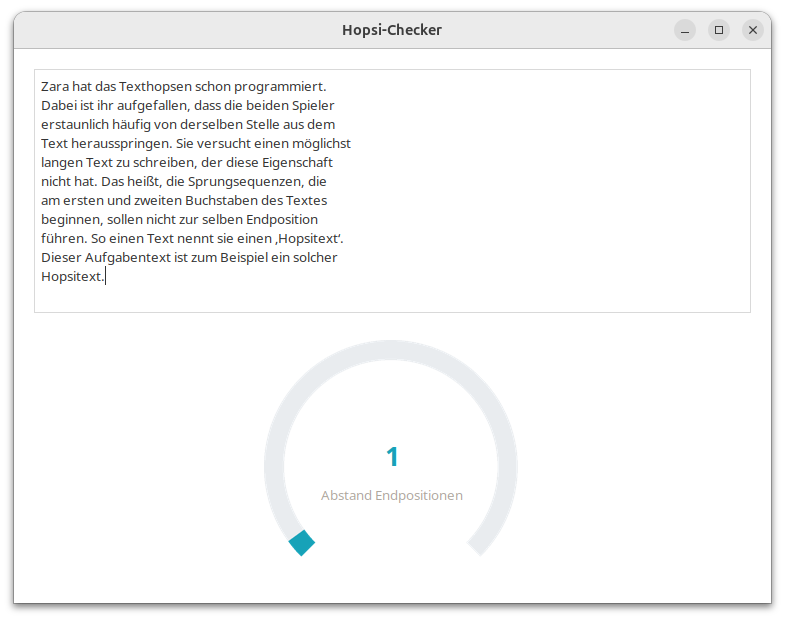
\includegraphics[width=0.7\linewidth]{Beispiel_BWINF_2}
	\caption{}
	\label{fig:beispielbwinf2}
\end{figure}


\section{Quellcode}
\begin{python}


from PIL import Image       # Image.CUBIC is deprecated (replaced by Image.BICUBIC)
Image.CUBIC = Image.BICUBIC # https://stackoverflow.com/a/76717474

import ttkbootstrap as ttk
from ttkbootstrap.constants import *
from ttkbootstrap.scrolled import ScrolledText
import threading
import time
import re


re_input = "" #erstelle Variable re_input
input = ""  #erstelle Variable input (notwendig da globale Variable)
abstand_endpositionen = 0 #erstelle Variable abstand_endpositionen


def sprungweite(buchstabe): # Nutze einen Index um die Sprungweite einen Buchstabens ueber die Position im Index +1 bestimmen zu können
    alphabet = ["a", "b", "c", "d", "e", "f", "g", "h", "i", "j", "k", "l", "m", "n", "o", "p", "q", "r", "s", "t", "u", "v", "w", "x", "y", "z", "ä", "ö", "ü", "ß"]
    return alphabet.index(buchstabe) + 1





def GUI():
    global input
    global re_input

    app = ttk.Window(title="Hopsi-Checker", themename="united")
    st = ScrolledText(app, padding=20, height=10, autohide=True) # erstelle Textfeld
    st.pack(fill=BOTH, expand=YES)    
    meter = ttk.Meter( # erstelle Radialanzeige
        metersize=260,
        padding=5,
        amountused=25,
        amounttotal=29,
        meterthickness=20,
        metertype="semi",
        subtext="Abstand Endpositionen",
        interactive=False,
        bootstyle="info",
        )
    meter.pack()

    while True:
        input = st.get("1.0",END) # hole den Text aus dem Textfeld und schreibe ihn in die variable input
        re_input = re.sub('[^A-Za-zäöüÄÖÜßẞ]', '', input) # Entfernt alle nicht-Buchstaben
        meter.configure(amountused = abstand_endpositionen) # Nutze Wert aus der Variable von abstand_endpositionen
        if abstand_endpositionen <= 5: # setze Farbe der Radialanzeige auf Rot wenn abstand_endpositionen <= 5
            meter.configure(bootstyle="danger")
        elif abstand_endpositionen >= 15: # setze Farbe der Radialanzeige auf Grün wenn abstand_endpositionen >= 15
            meter.configure(bootstyle="success")
        else:
            meter.configure(bootstyle="info")
        app.update() # update the GUI
        


def check_hopsi(Startposition):
    global abstand_endpositionen
    not_finished = True #setze Variiable not_finished auf True
    Stelle = Startposition

    while not_finished == True:
        lt_re_input = list(re_input.lower()) # Wandelt ipnut in Liste um und wandelt alle Buchstaben in Kleinbuchstaben um
        if len(lt_re_input) <= 1:
            abstand_endpositionen = 0
            time.sleep(0.5)
        else:
            if sprungweite(lt_re_input[Stelle]) + Stelle < len(lt_re_input):
                Stelle = Stelle + sprungweite(lt_re_input[Stelle])
            else:
                not_finished = False
    return Stelle


def berechne_differenz(Wert1, Wert2): #Funktion zur Berechnung der Differenz von zwei positiven Werten
    if Wert1 > Wert2:
        Wert_diff = Wert1 - Wert2
    else:
        Wert_diff = Wert2 - Wert1
    return Wert_diff


def check_all():
    time.sleep(0.5)
    global abstand_endpositionen
    while True:
        time.sleep(0.1)
        check_hopsi(0)
        check_hopsi(1)
        abstand_endpositionen = berechne_differenz(check_hopsi(0), check_hopsi(1))



t1_GUI = threading.Thread(target=GUI) 
t2_check_hopsi = threading.Thread(target=check_all)
t1_GUI.start()
t2_check_hopsi.start()
\end{python}
\end{document}